
%(BEGIN_QUESTION)
% Copyright 2012, Tony R. Kuphaldt, released under the Creative Commons Attribution License (v 1.0)
% This means you may do almost anything with this work of mine, so long as you give me proper credit

\centerline{\bf The Rules of \underbar{Fault Club}}

\begin{itemize}
\item{$(1)$} Don't try to find the fault by looking for it -- perform diagnostic tests instead
\vskip 10pt
\item{$(2)$} {\it Don't try to find the fault by looking for it -- perform diagnostic tests instead!}
\vskip 10pt
\item{$(3)$} The troubleshooting is over when you have correctly identified the nature and location of the fault
\vskip 10pt
\item{$(4)$} It's just you and the fault -- don't ask for help until you have exhausted your resources
\vskip 10pt
\item{$(5)$} Assume one fault at a time, unless the data proves otherwise
\vskip 10pt
\item{$(6)$} No new components allowed -- replacing suspected bad components with new is a waste of time and money
\vskip 10pt
\item{$(7)$} We will practice as many times as we have to until you master this
\vskip 10pt
\item{$(8)$} Troubleshooting is not a spectator sport: \underbar{\it you} have to troubleshoot!
\end{itemize}

\vskip 10pt

These rules are guaranteed to help you become a better troubleshooter, and will be consistently emphasized by your instructor.


\filbreak

\noindent
{\bf Loop diagram template}

$$\includegraphics[width=15.5cm]{i00654x01.eps}$$

\vfil \eject

\noindent
{\bf Loop diagram requirements}

Perhaps the most important rule to follow when drafting a loop diagram is {\it your diagram should be complete and detailed enough that even someone who is not an instrument technician could understand where every wire and tube should connect in the system!}

\begin{itemize}
\item{} {\bf Instrument ``bubbles''}
\item{} Proper symbols and designations used for all instruments.
\item{} All instrument ``bubbles'' properly labeled (letter codes and loop numbers).
\item{} All instrument ``bubbles'' marked with the proper lines (solid line, dashed line, single line, double lines, no lines).
\item{} {\it Optional:} Calibration ranges and action arrows written next to each bubble.
\end{itemize}

\begin{itemize}
\item{} {\bf Text descriptions}
\item{} Each instrument documented below (tag number, description, etc.).
\item{} Calibration (input and output ranges) given for each instrument, as applicable.
\end{itemize}

\begin{itemize}
\item{} {\bf Connection points}
\item{} All terminals and tube junctions properly labeled.
\item{} All terminal blocks properly labeled.
\item{} All junction (``field'') boxes shown as distinct sections of the loop diagram, and properly labeled.
\item{} All control panels shown as distinct sections of the loop diagram, and properly labeled.
\item{} All wire colors shown next to each terminal.
\item{} All terminals on instruments labeled as they appear on the instrument (so that anyone reading the diagram will know which instrument terminal each wire goes to).
\end{itemize}

\begin{itemize}
\item{} {\bf Cables and tubes}
\item{} Single-pair cables or pneumatic tubes going to individual instruments should be labeled with the field instrument tag number (e.g. ``TT-8'' or ``TY-12'')
\item{} Multi-pair cables or pneumatic tube bundles going between junction boxes and/or panels need to have unique numbers (e.g. ``Cable 10'') as well as numbers for each pair (e.g. ``Pair 1,'' ``Pair 2,'' etc.).
\end{itemize}

\begin{itemize}
\item{} {\bf Energy sources}
\item{} All power source intensities labeled (e.g. ``24 VDC,'' ``120 VAC,'' ``20 PSI'')
\item{} All shutoff points labeled (e.g. ``Breaker \#5,'' ``Valve \#7'')
\end{itemize}

\vfil \eject

\noindent
{\bf Sample Loop Diagram (using a single-loop controller)}

$$\includegraphics[width=15.5cm]{i00654x02.eps}$$


\vfil \eject

\noindent
{\bf Sample Loop Diagram (using DCS controller)}

$$\includegraphics[width=15.5cm]{i00654x03.eps}$$


\vfil \eject

\noindent
{\bf Sample Loop Diagram (using pneumatic controller)}

$$\includegraphics[width=15.5cm]{i00654x04.eps}$$


\vfil \eject

\noindent
{\bf Sample Loop Diagram (using PLC, with electronic positioner installed on valve)}

$$\includegraphics[width=15.5cm]{i00654x05.eps}$$

\underbar{file i00654}
%(END_QUESTION)





%(BEGIN_ANSWER)

Your loop diagram will be validated when the instructor inspects the loop with you and the rest of your team.

%(END_ANSWER)





%(BEGIN_NOTES)


%INDEX% Lab exercise, loop diagram template and requirements

%(END_NOTES)


